\documentclass[11pt,a4paper]{article}
\usepackage{tabularx}
\usepackage[english]{babel}
\usepackage{array}
\usepackage{graphicx}
\usepackage{color}
\DeclareGraphicsExtensions{.eps,.png,.pdf,.ps}
\begin{document}
\title{Summary reports of non-classic function detection of : test5}

\vspace{-1cm}
\maketitle
\tableofcontents
\newpage
\newpage
\section{Data description}
\begin{quotation}
Table 1 mainly describes the input files, parameters and options.
\end{quotation}
\begin{table}[h]
\caption{parameter description}\label{bstable}
\begin{tabularx}{\textwidth}{ |X|l| }

      
\hline
parameter & value  \\
\hline
output name & test5 \\
\hline
HMRpeak(peak filename) & mESC\_GSM1562337\_CBX7.bed \\
\hline
HM signal(bw filename) & mESC\_GSM1399500\_H3K27me3.bw  \\
\hline
\#coTF candidates & 143 \\
\hline
options & value \\
\hline
extend size & 1000bp \\
\hline
Alpha (Elastic net) & 0.5 \\
\hline
Pvalue cutoff & 0.001 \\
\hline
topN cofactors & all \\
\hline

\end{tabularx}
\end{table}

\newpage
\newpage
\section{ElasticNet co-factor selection}
In this step we use a feature selection (elastic-net. Zou, H. and Hastie T. (2005) to select potential co-factors which corresponded to the non-classic function. Below shows the cross-validation curve for the decison of lambda in elastic-net.  
\begin{figure}[h]
        \caption{cross-validation curve for lambda decision} \label{fig:profileunion}
        \setlength{\abovecaptionskip}{0pt}
        \setlength{\belowcaptionskip}{10pt}
        \centering
        {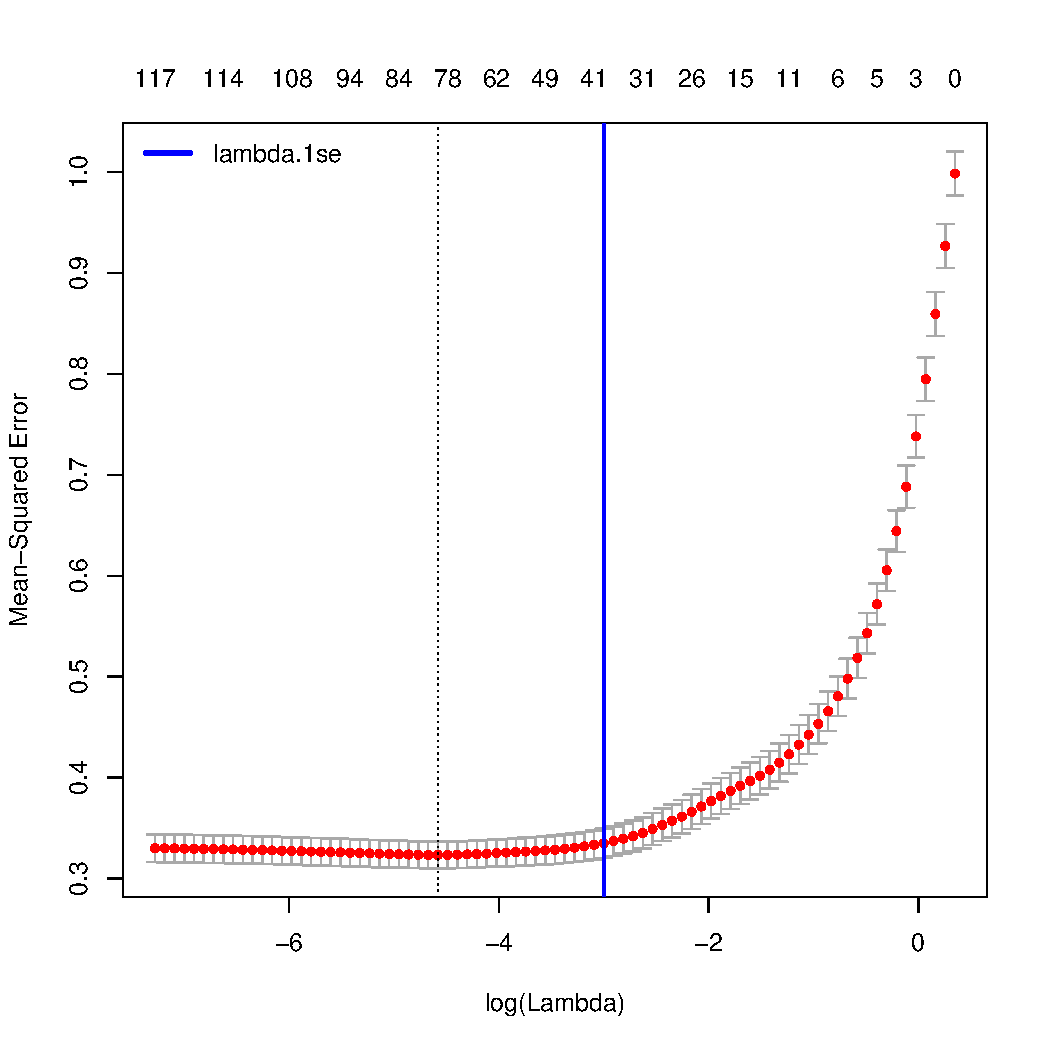
\includegraphics[width=0.8\textwidth]{test5_elnet_lambdaSelection.pdf}}
\end{figure}

\newpage
\newpage
\section{potential co-factors corresponded to non-classic function}
In summary, 9 factors were predicted to potentially act as a co-factor of the non-classic function. The top9 co-factors were listed.
\subsection{summary of co-factors}
\begin{quotation}
The empirical p-value, R-square (ordered) and the number of non-classic (NC) sites for each potential co-factors were listed below. The empirical p-value was calculated based on the comparison of foreground (observed) R-square and background R-square (distribution of random R-square generated from the 1,000 permutations of co-binding events) for each potential co-factor. The non-classic sites were defined by lower HM signal (using Otus' method) and co-binding events of each potential co-factor.
\end{quotation}
\begin{table}[h]
\caption{cofactor summary}\label{bstable}
\begin{tabularx}{\textwidth}{ |l|X|X|X| }
    
\hline
co-factor & p-value & R-square & \#NCsites \\
\hline
mESC\_GSM1842750\_NANOG & 0.001 & 0.503 & 1211 \\
\hline
mESC\_GSM1355157\_OTX2 & 0.001 & 0.372 & 1015 \\
\hline
mESC\_GSM623989\_PRDM14 & 0.001 & 0.357 & 1001 \\
\hline
mESC\_GSM1258240\_ASH2L & 0.001 & 0.301 & 922 \\
\hline
mESC\_GSM1355154\_POU5F1 & 0.001 & 0.235 & 1079 \\
\hline
mESC\_GSM1208218\_KLF5 & 0.001 & 0.169 & 761 \\
\hline
mESC\_GSM1406445\_TRIM28 & 0.001 & 0.124 & 568 \\
\hline
mESC\_GSM1003807\_ZNF384 & 0.001 & 0.106 & 483 \\
\hline
mESC\_GSM935891\_ELL3 & 0.001 & 0.105 & 459 \\

\hline
\end{tabularx}
\end{table}
\newpage
\newpage
\subsection{Boxplot of HM on non-classic and classic sites}
\begin{quotation}
Boxplot was generated to compare the difference of the histone mark (HM) signal on either non-classic(NCpeak) or classic sites. The non-classic sites were defined by lower HM signal (using Otus' method) and co-binding events of each potential co-factor. The boxplot corresponded to top5 co-factors were displayed.  
\end{quotation}
\begin{figure}[h]
        \caption{boxplot cofactor HMsignal} \label{fig:profileunion}
        \setlength{\abovecaptionskip}{0pt}
        \setlength{\belowcaptionskip}{10pt}
        \centering
        {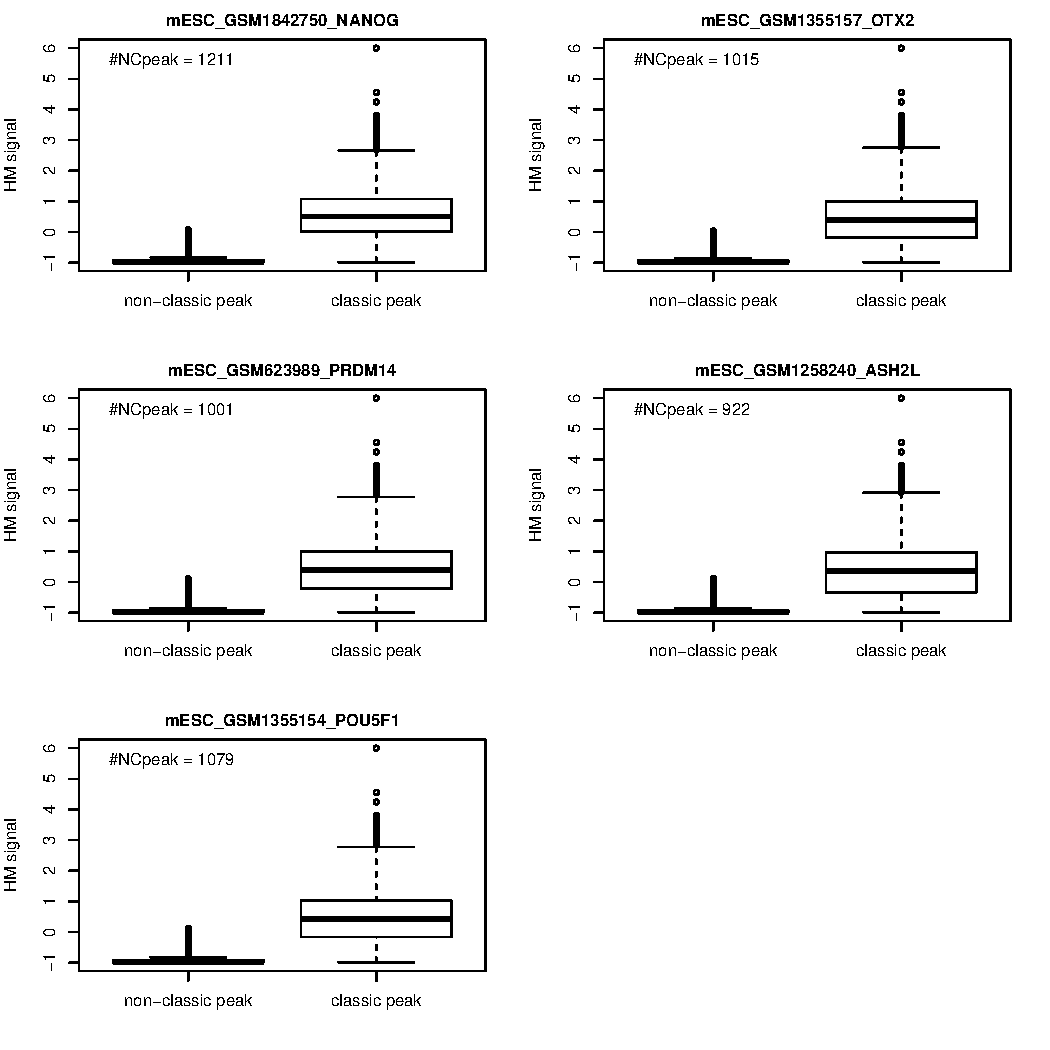
\includegraphics[width=0.8\textwidth]{test5_coTF_HMsignal.pdf}}
\end{figure}

\newpage
\newpage
\section{Output list}
\begin{quotation}
All output files were described in the following table
\end{quotation}
\begin{table}[h]
\caption{output list}\label{bstable}
\begin{tabularx}{\textwidth}{ |X|l| }
    
\hline
description & filename \\
\hline
cobinding matrix on HMR peaks & tmpResults/test5\_peakov.bed \\
\hline
histone mark signal on HMR peaks & tmpResults/test5\_HMsig.bed \\
\hline
summary table of non-classic function & summary/test5\_NCsummary.txt \\
\hline
summary report (this doc) & summary/test5\_summary.pdf \\
\hline

\end{tabularx}
\end{table} 
\end{document} 

